\title{Lupus in Tabula}
\author{Edoardo Morassutto}

\documentclass[10pt,a4paper]{article}
\usepackage[utf8]{inputenc}
\usepackage[italian]{babel}
\usepackage{amsmath}
\usepackage{amsfonts}
\usepackage{amssymb}
\usepackage{hyperref}		% pacchetto per i link
\usepackage{color}			% pacchetto per colorare il testo
\usepackage{graphicx}		% pacchetto per includere le immagini
\usepackage{svg}				% pacchetto per includere le immagini vettoriali
\usepackage{amsmath}

% rimuove indentazione e aggiunge 3pt di spazio tra i paragrafi
\setlength{\parindent}{0pt}
\setlength{\parskip}{3pt}

\newcommand{\ruolobuono}[1]{
{\color{green}{\textbf{#1}}}
}
\newcommand{\ruolocattivo}[1]{
{\color{red}{\textbf{#1}}}
}
\newcommand{\manabuono}{
{\color{green}{$\star$}}
}
\newcommand{\manacattivo}{
{\color{red}{$\star$}}
}
\begin{document}
\maketitle

Tutto il sorgente è disponibile all'indirizzo: \url{https://github.com/lupus-dev/lupus}

Per contattare l'amministratore: \url{edoardo.morassutto@gmail.com}

Puoi contattarmi su Facebook se mi hai tra gli amici!

Se vuoi dare una mano ogni tanto forka il repository /lupus-dev/lupus su GitHub e inviaci una Pull Request, se sei stato bravo la mergiamo volentieri!

Se vuoi diventare uno sviluppatore chiedimelo e vedrò di accontentarti!

\section{Introduzione}
Il progetto viene scritto in PHP. Ovviamente non può mancare l'HTML, JavaScript, CSS, database, git, SASS, ed altro...

\subsection{Pacchetti software}
Il progetto verrà avviato su una macchina con questi pacchetti (e dipendenze):
\begin{itemize}
\item Apache2 (qualunque versione recente dovrebbe andare)
	\begin{itemize}
	\item Mod\_rewrite (necessaria per il rewrite dell'url)
	\end{itemize}
\item PHP 5.3 (compatibile con i più comuni webserver gratuiti)
	\begin{itemize}
	\item estensioni varie da definire (le solite comunque)
	\end{itemize}
\item MySQL (compatibile con i più comuni webserver gratuiti)
\item SASS (solo lato compilazione del CSS)
	\begin{itemize}	
	\item Quindi Ruby...	
	\end{itemize}
\end{itemize}

\subsection{Motivazione delle scelte}
\subsubsection*{Apache2}
Ormai questo è un must dei webserver, nulla da ridire, facile da configurare, veloce, compatibile con tutti i servizi di webhosting gratuiti. 

È necessario abilitare l'estensione mod\_rewrite (solitamente è già attiva) per consentire il rewrite degli indirizzi e rendere più accattivante il servizio del gioco.

Tramite il file .htaccess vengono configurate l'estensioni usate, facile il verisioning e la gestione della configurazione

\subsubsection*{PHP}
Dato che il server del gioco verrà scritto in PHP, è necessario che PHP sia installato e configurato correttamente. 

Il progetto verrà scritto in PHP 5.3 (la versione attuale di Altervista) per permettere una facile migrazione di host nel caso sia necessario e per renderlo il più retrocompatibile possibile. Alcune funzioni sono state marcate come “deprecated” in 5.4, sapendolo cerchiamo di evitarle... Ad esempio non useremo l'estensione mysql ma la nuova mysqli con approccio ad oggetti. È necessario quindi che sia abilitata se non lo fosse già.

\subsubsection*{MySQL}
Per quanto mi possa piacere di più PostgreSQL sono costretto a scegliere di usare MySQL per le stesse ragioni per cui useremo PHP 5.3. PostgreSQL non è supportato da Altervista e da altri webhosting gratuiti. La versione è abbastanza ininfluente, non useremo funzioni particolarmente recenti.

\subsubsection*{SASS}
SASS è un preprocessore di CSS, permette di scrivere il CSS molto più semplicemente e di applicare delle particolari formattazioni al file .css in maniera del tutto automatica. Le più importanti differenze tra CSS e SASS sono:
\begin{itemize}
\item In SASS si possono dichiarare le variabili ed effettuare operazioni con esse
\item Si può decidere di comprimere il file .css di output 
\item Si possono annidare le dichiarazioni (vedi manuale del SASS)
\item È molto più facile da leggere e da mantenere
\item Si possono includere altri fogli SASS dentro un file SASS (aka import)
\end{itemize}

SASS richiede che sia installato anche Ruby per funzionare... 

Usando NetBeans è possibile abilitare la compilazione automatica e trasparente dei file .scss ad ogni salvataggio.

\newpage

\section{Il gioco}
Lupus in Tabula è un gioco di ruolo molto complesso. Per imparare a giocare si può fare riferimento al nostro amato amico Google.

Questa è una semplice guida per iniziare a giocare:

\url{http://www.davincigames.net/lit/lupus_in_tabula_4th_regole.pdf}

Ignorare a prescindere la roba delle carte e pensare in grande per scrivere un server web...

\subsection{Struttura dei componenti}
Ovviamente perché si possa chiamare “gioco” è necessario che tutto abbia una struttura solida e chiara. Vengono quindi spiegate le principali entità del gioco. Tutti i riferimenti ai nomi brevi sono chiariti nella sezione apposita.

\subsubsection{Gli utenti}
\begin{itemize}
\item Ogni utente che si registra ha un identificativo univoco che fa da chiave primaria
\item Ogni utente ha uno \textsf{username} univoco che usa per identificarsi e per accedere al sito
\item Lo \textsf{username} è un nome breve
\item Ogni utente ha un livello pubblico che determina i privilegi a cui l'utente può accedere
\item Ogni utente ha una email che viene usata per verificare l'account e notificare qualcosa... Da definire
\end{itemize}

\subsubsection{Le stanze}
\begin{itemize}
\item Ogni utente di livello appropriato può creare un certo numero di stanze (in base al livello)
\item Ogni stanza può contenere più partite, una sola però può essere attiva
\item Ogni stanza ha un nome breve \textsf{room\_name}
\item Ogni stanza ha una descrizione con lo stesso grado di accessibilità della partita
\item Le stanze possono essere private o pubbliche
\item Ogni utente può visualizzare una stanza pubblica
\item Solo gli utenti partecipanti e/o autorizzati possono visualizzare una stanza privata
\item Ogni stanza ha un amministratore, colui che ha creato la stanza
\item Le stanze possono essere eliminate
\end{itemize}

\subsubsection{Le partite}
\begin{itemize}
\item Ogni partita è interna ad una stanza
\item Ogni partita ha un nome breve unico per quella stanza (\textsf{game\_name})
\item Ogni partita ha un titolo scelto dall'amministratore
\item L'amministratore della partita è l'amministratore della stanza corrispondente
\item Possono essere create delle partite solo se non ci sono partite attive
\item Gli utenti possono essere invitati nella partita oppure possono richiedere all'amministratore di farne parte
\item La partita può iniziare solo se è presente il numero minimo di giocatori
\item La partita viene avviata dall'amministratore
\item L'amministratore può espellere un giocatore
\item L'amministratore può terminare la partita
\item Lo stato della partita e i ruoli dei giocatori vengono rilevati solo al termine della partita
\item La chat della partita rimane visibile solo ai giocatori
\item Eventuali altre chat vengono disabilitate alla fine della partita
\end{itemize}

\subsubsection{I livelli}
\begin{itemize}
\item Ogni utente ha un livello
\item Il livello è solo crescente (non si può essere degradati tranne dall'game master)
\item Un utente bannato ha livello uguale a zero
\end{itemize}

\subsubsection{Nomi brevi}
Tutti i riferimenti ai nomi brevi sono da intendere che rispettano le seguenti caratteristiche:
\begin{itemize}
\item Hanno una lunghezza di al più 10 caratteri
\item Sono formati da soli caratteri ASCII alfanumerici minuscoli/cifre
\item Il primo carattere è una lettera
\item Ogni nome breve è unico rispetto al proprio contesto
\end{itemize}

\subsection{Struttura del server}
\subsubsection*{Modulare}
Il server (forse le API) sono gestite nel modo più modulare possibile:

Deve essere possibile avere una cartella dove mettere dei file php contenenti i ruoli. Aggiungere e togliere dei ruoli deve essere una semplice modifica del relativo file in questa cartella. 

Non deve essere presente un file dove vengono registrati i ruoli, deve essere gestito in maniera automatica e dinamica.

\subsubsection*{Orientato agli oggetti}
Ogni ruolo deve essere un oggetto che deriva dalla classe \textsf{Ruolo}

Il server include tutti i ruoli presenti nella cartella dedicata. Ognuno di questi file contiene una classe e un'istruzione del genere:
\begin{verbatim}
$ruoli[] = "nomeClasse";
\end{verbatim}

Dove \textsf{\$ruoli} è un vettore che conterrà i nomi delle classi da interpretare come ruoli. Se uno dei file in quella cartella non dovesse contenere quell'istruzione allora quel ruolo non sarà abilitato.

Se un giocatore ha un ruolo non esistente o non abilitato la partita termina a causa di un errore interno.

\subsection{Ruoli}
I ruoli da implementare fin da subito potrebbero essere: (il colore indica la fazione, la stella il mana)
\begin{itemize}
\item \ruolocattivo{Lupo\manacattivo} Durante la notte i lupi votano chi eliminare, se almeno il 50\%+1 dei lupi vivi votano la stessa persona, questa è una candidata a morire
\item \ruolobuono{Guardia\manabuono} Durante la notte la guardia può scegliere di proteggere una persona, se i lupi quella notte decidessero di ucciderla, essa non muore.
\item \ruolobuono{Medium\manabuono} Il medium durante la notte può scegliere di guardare un giocatore morto, lui saprà se quel giocatore aveva un mana buono o cattivo.
\item \ruolobuono{Veggente\manabuono} Il veggente può fare le stesse operazioni del medium, solo sui giocatori vivi.
\item \ruolobuono{Paparazzo\manabuono} Il paparazzo durante la notte sceglie una persona da pedinare, vengono riportati sul giornale della mattina tutti i giocatori che hanno visitato il paparazzato.
\item \ruolobuono{Criceto mannaro\manacattivo} \'E un giocatore normale, senza poteri speciali. Se la partita termina e lui è ancora vivo allora vince solo lui e non la sua fazione.
\item \ruolobuono{Assassino\manacattivo} L'assassino una sola volta nella partita può scegliere una persona e ucciderla
\item \ruolobuono{Massone\manabuono} I massoni non hanno poteri però hanno una chat dedicata e quindi si conoscono tra loro
\item \ruolobuono{Contadino\manabuono} I contadini non hanno poteri...
\item \ruolobuono{Pastore\manabuono} I pastori possono scegliere di sacrificare delle pecore per salvare dei giocatori dalle grinfie dei lupi
\item \ruolobuono{Falso\manacattivo} Il falso può scegliere tra una serie di proposizioni false e renderle pubbliche sul giornale
\item \ruolobuono{Prescelto\manabuono} Il prescelto all'inizio della partita conosce 4 proposizioni, 2 vere e 2 valse
\item \ruolobuono{Sindaco\manabuono} Il sindaco è un contadino che non può essere messo al rogo
\end{itemize}

\section{Il server}
Il server è suddiviso in più parti:
\begin{itemize}
\item Il database
\item Le API
\item La web-app
\end{itemize}

\subsection{Il database}
Il database è formato da una serie di tabelle spiegate nel dettaglio nella sezione dedicata più avanti

\subsection{Le API}
A causa della natura dinamica del gioco sono necessarie delle funzioni accessibili facilmente tramite JavaScript. Tramite queste funzioni è possibile far proseguire la partita, ottenere informazioni ed effettuare richieste al server.

\subsection{La web-app}
L'interfaccia grafica del gioco sarà sviluppata con la libreria BootStrap, la quale rende tutto molto portabile su dispositivi con schermo ridotto. 

Non ci sarà troppo PHP in queste pagine, il grosso del lavoro sarà il JavaScript a farlo in coppia con le API.

\subsubsection*{Pagine}
Quello che segue è un elenco delle pagine che devono essere implementate
\begin{itemize}
\item \textsf{/login} è la pagina per accedere al sito
\item \textsf{/admin} è una pagina che contiene la lista dei collegamenti alle altre pagine di amministrazione 
\item \textsf{/admin/(room\_name)} è la pagina di amministrazione di una stanza
\item \textsf{/admin/(room\_name)/(num$|$game\_name)} è la pagina di amministrazione di una partita
\item \textsf{/game} è una pagina che contiene la lista dei collegamenti alle altre pagine di gioco
\item \textsf{/game/(room\_name)} è una pagina che contiene le partite di una stanza
\item \textsf{/game/(room\_name)/(num$|$game\_name)} è la pagina di gioco di una partita
\item \textsf{/user} è la pagina dell'utente
\item \textsf{/user/(username)} è la pagina di un utente specifico
\item \textsf{/status} contiene lo stato del server (numero di partite, di stanze, ecc...)
\item \textsf{/join} è la pagina per trovare una partita
\item \textsf{/singup} è la pagina per registrarsi
\end{itemize}

\newpage

\section{Il database}
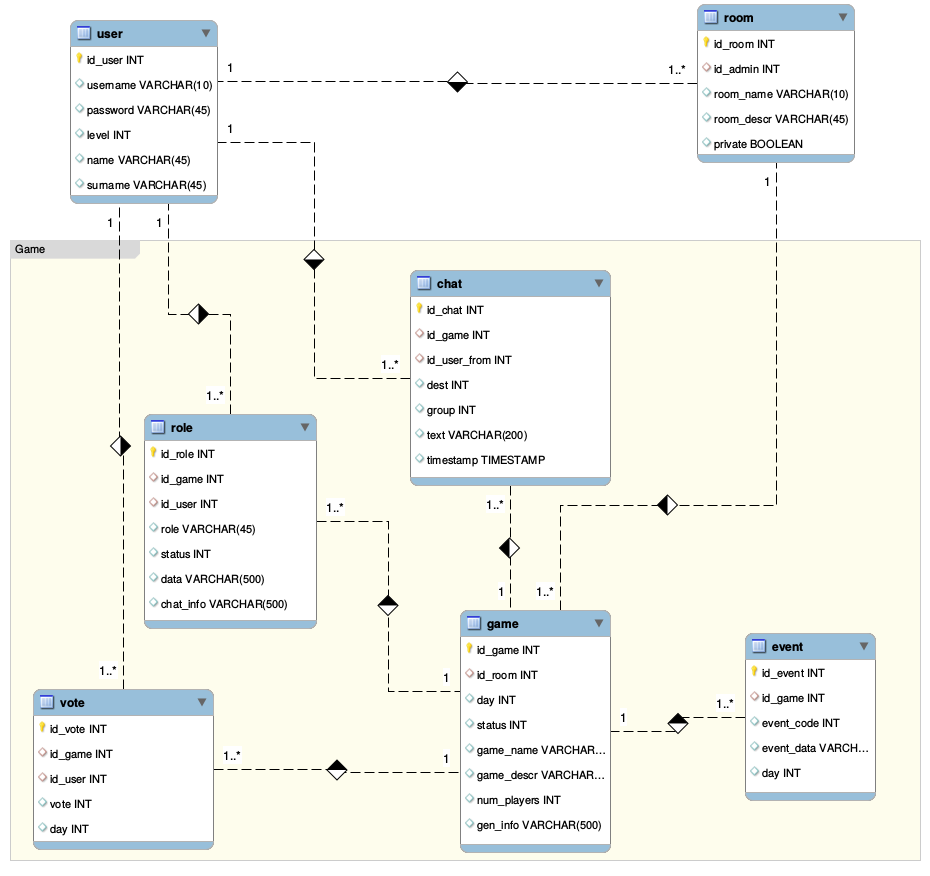
\includegraphics[width = \textwidth]{database.png}

Questa è una bozza della struttura del database, ci saranno sicuramente molte modifiche. Lo schema E-R è stato disegnato con il programma \textsf{MySQL Workbench}.

\subsection{Tabella user}
In questa tabella vengono memorizzati gli utenti registrati. Ogni utente ha un \textsf{id\_user} che rimane nascosto al pubblico e identifica all'interno del database uno ed un solo utente. Ogni utente è identificato all'esterno con un \textsf{username} unico che rispetta il formato "nome breve"

La password dell'utente è salvata codificata in SHA-256. In futuro potrebbe essere aggiunto un ulteriore livello di protezione aggiungendo del salt.

Il livello dell'utente è salvato nella righe dell'utente. Ogni volta che si verifica un evento che potrebbe modificare il livello, si ricalcola il livello e lo si aggiorna solo se è strettamente maggiore.

\subsection{Tabella room}
La tabella \textsf{room} contiene le informazioni di una stanza. Ogni stanza ha un identificativo univoco \textsf{id\_room}, nascosto al pubblico che identifica la stanza all'interno del database. Ogni stanza contiene l'identificativo dell'utente amministratore della stanza \textsf{id\_admin}. Al pubblico la stanza è identificata con un nome \textsf{room\_name} il quale è unico. Ogni stanza ha anche una descrizione \textsf{room\_descr} che rappresenta il titolo della stanza. 

Il campo \textsf{open} nelle prime versioni sarà ignorato perché vanno definiti ancora i permessi per la creazione di stanze e di partite.

\subsection{Tabella game}
La tabella game raccoglie le informazioni di una singola partita. Ogni partita è identificata all'interno del database con un identificativo unico \textsf{id\_game}. Ogni partita è contenuta all'interno di una stanza \textsf{id\_room}. Ogni partita è identificata all'esterno con un nome breve unico all'interno della stessa stanza \textsf{game\_name}, inoltre ogni partita ha una descrizione che rappresenta il titolo della partita \textsf{game\_descr}.

I campi \textsf{day} e \textsf{status} sono informazioni utili della partita, l'istante temporale del gioco e lo stato della partita (in corso, terminata, interrotta, ecc...)

\subsection{Tabella role}
In questa tabella sono memorizzati i ruoli dei giocatori interni ad una partita. Ogni riga è identificata da un campo \textsf{id\_role} non pubblico. Ogni ruolo è interno alla partita \textsf{id\_game} e relativo all'utente \textsf{id\_user}. 

Il ruolo dell'utente è memorizzato nella stringa \textsf{role} la quale identifica un ruolo nella cartella dei ruoli. Il campo \textsf{status} indica lo stato dell'utente (vivo, morto, ecc...). Alcuni ruoli potrebbero richiedere di memorizzare delle informazioni aggiuntive, il campo \textsf{data} contiene dei dati salvati da un ruolo, codificati in \textsf{JSON}.

\subsection{Tabella vote}
In questa tabella vengono memorizzati i voti degli utenti. Ogni voto è identificato tramite il campo \textsf{id\_vote}, il quale rimane nascosto all'esterno del database. Ogni voto è specifico della partita \textsf{id\_game} nel momento \textsf{day} e appartiene all'utente \textsf{id\_user}. Il suo voto è \textsf{vote} il quale può essere l'identificativo di un utente ma anche altro. 

\subsection{Tabella chat}
In questa tabella vengono memorizzati i messaggi delle varie chat. Ogni messaggio è identificato all'interno del database da \textsf{id\_chat}. Ogni messaggio si riferisce alla partita \textsf{id\_game}. Il mettente del messaggio è \textsf{id\_user\_from} cioè l'identificativo dell'utente che ha inviato il messaggio. Il destinatario \textsf{to} è un numero intero che può rappresentare vari identificativi, in base a \textsf{level} il destinatario può essere un utente, il pubblico, una chat privata, ecc..

Il testo del messaggio è \textsf{text} il quale non può essere più lungo di 200 caratteri e viene eseguito l'escape sia per il database che per il JavaScript.

\subsection{Tabella newspaper}
In questa tabella viene memorizzato il giornale dei vari giorni della partita. Ogni articolo è identificato da \textsf{id\_news} ed appartiene alla partita \textsf{id\_game} al tempo \textsf{day}. Il testo dell'articolo è memorizzato in \textsf{news}.

\newpage
\tableofcontents

\end{document}